\section{MF Ranking Model}
\label{chap:tree-ranking:mf-model}

In this section we present the multi-valued attribute ranking model, denoted with ``MF''. It generalizes field-based ranking models to arbitrary trees.
First, we present the revised entity model and introduce the formal model of MF. Next we present two extensions to the MF model. Finally, we describe weights developed for the MF model.

\subsection{Tree Model}

In general, an entity contains some structure which provides relevant information about its content. For example, an entity that describes a book would be divided into chapters, each chapter into sections, each section into a set of paragraphs. In order to retain this structure for later use in the ranking, we need to generalize the entity model presented in \ref{chap:entity-ranking:entity-model} into a tree of arbitrary height and varying degree.

The Figure~\ref{fig:concept-tree} depicts an entity as a tree. Each node identified from $a$ to $g$ contains possibly some textual content.
Compared to the entity model presented in \ref{chap:entity-ranking:entity-model}, an entity is then represented by the root of the tree. We refer to \emph{attribute} and \emph{value} as internal nodes instead.
As a parallel with RDF data, the node $a$ is the ``subject'' of the entity, the nodes $b$ and $d$ its predicates, the nodes $c$, $e$ and $f$ the objects, and $g$ the predicate of the object $e$.

\subsection{MF Model Normalisations}
\label{chap:tree-ranking:mf-model:norm}

In traditional field-based ranking models, most of the structure of the entity is discarded. BM25F integrates some structure into its model by defining ``fields''. A field is a collection of words, or a \emph{bag of words}, where the words are related to a same topic. However, the bag of words representation of a field loses the structure the content of the field might have. In order to capture this structure and to integrate the degree variability into the ranking function itself, we model a field not as a bag of words but as a bag of \emph{bags}, where each bag can be a bag of words or also a bag of bags.

With a traditional field-based ranking model, the content of each field loses its structure. As depicted in Figure~\ref{fig:field-model}, the nodes are agglomerated into a bag of words within a field, represented as squares. The content of the root node $a$ may also contribute to the ranking of the entity by defining another field, called ``entity'' in the figure, which contains the content of the node $a$. The contribution of a query term is first computed for each field, then each contribution is aggregated into a final score for the entity, depicted by the $*$ node in the figure.

Instead, the contribution of a query term in the MF model sticks to the structure of the entity: the contribution is computed on the leaves, then it is aggregated at each internal node up to the root. In order to take into consideration the content of an internal node into the ranking, we need to transform the tree so that an internal node becomes a leaf. The internal node is then replaced by a content-less node, which purpose is to aggregate the contributions of its sub-tree. The Figure~\ref{fig:mf-model} depicts the MF model applied on the entity tree, with a square symbolizing where the contribution of a query term is performed, and red dashed squares representing internal nodes in the entity tree that were transformed into a leaf.

The contribution of a query term is then computed starting on the leaves, which is aggregated on the parent node; if the parent node is not the root, its contribution will be aggregated along with the contributions of its siblings. The entity score is then derived by combination across the terms. The MF ranking model leads then to a new definition of the term frequency normalization function in field-based ranking models. For example, the computation starts on the nodes $e$ and $g$ in the figure, which contribution is aggregated on the parent node. This contribution is aggregated along with those of the nodes $d$ and $f$. Finally, this contribution is aggregated with those of the other branches into a final score for the entity.

In the MF ranking model, a leaf is a node that possesses textual content, and an internal node purpose is to aggregate the contribution of its children. Therefore, we apply the normalisation logic regarding the term frequency on a leaf, e.g., normalisation to the field length in BM25F. The internal nodes allow to add an additional normalisation step that captures the degree variability.

\begin{figure}[t]
    \centering
    \begin{subfigure}{0.3\textwidth}
    	\centering
      	\begin{tikzpicture}
\node (a) at (-.25,0) {a};
\node (b) at (-1,-1) {b};
\node (c) at (-1,-2) {c};
\node (d) at (0.5,-1) {d};
\node (e) at (0,-2) {e};
\node (f) at (1,-2) {f};
\node (g) at (0,-3) {g};
\draw (a) -- (b) -- (c);
\draw (a) -- (d) -- (e) -- (g);
\draw (a) -- (d) -- (f);
\end{tikzpicture}
    	\caption{An entity represented as a tree with varying degree.}
		\label{fig:concept-tree}
    \end{subfigure}
  	\quad
  	\begin{subfigure}{0.3\textwidth}
  		\centering
  		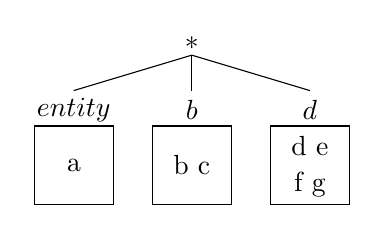
\begin{tikzpicture}
% field entity
\node at (-1,1.2) {$entity$};
\node at (-1,.5) {a};
\draw (-1.5,0) rectangle (-.5,1);
% field b
\node at (.5,1.2) {$b$};
\node at (.5,.5) {b c};
\draw (0,0) rectangle (1,1);
% field d
\node at (2,1.2) {$d$};
\node at (2,.75) {d e};
\node at (2,.25) {f g};
\draw (1.5,0) rectangle (2.5,1);
% Aggregate contributions of each field
\node at (.5,2) {*};
\draw (.5,1.9) -- (-1,1.45);
\draw (.5,1.9) -- (.5,1.45);
\draw (.5,1.9) -- (2,1.45);
\end{tikzpicture}
  		\caption{Field-based ranking model for the entity. The $*$ symbolises the aggregation of the contribution of each child node, here a field.}
		\label{fig:field-model}
  	\end{subfigure}
  	\quad
  	\begin{subfigure}{0.3\textwidth}
  		\centering
  		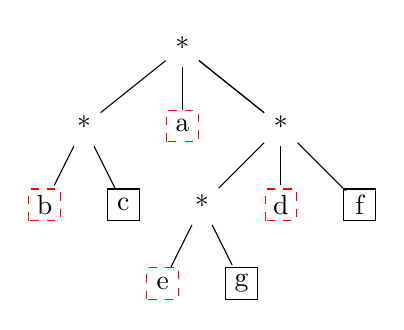
\begin{tikzpicture}
\node (a) at (-.25,0) {*};
\node (labela) at (-.25,-1) {a};
\node (b) at (-1.5,-1) {*};
\node (labelb) at (-2,-2) {b};
\node (c) at (-1,-2) {c};
\node (d) at (1,-1) {*};
\node (labeld) at (1,-2) {d};
\node (e) at (0,-2) {*};
\node (labele) at (-.5,-3) {e};
\node (f) at (2,-2) {f};
\node (g) at (.5,-3) {g};

\draw (a) -- (labela);
\draw (a) -- (b) -- (c);
\draw (b) -- (labelb);
\draw (d) -- (labeld);
\draw (e) -- (labele);
\draw (a) -- (d) -- (e) -- (g);
\draw (a) -- (d) -- (f);

\draw [red, dashed] (-2.2,-2.2) rectangle (-1.8,-1.8);
\draw (-1.2,-2.2) rectangle (-.8,-1.8);
\draw [red, dashed] (-.45,-1.2) rectangle (-.05,-.8);
\draw [red, dashed] (.8,-2.2) rectangle (1.2,-1.8);
\draw (1.8,-2.2) rectangle (2.2,-1.8);
\draw [red, dashed] (-.7,-3.2) rectangle (-.3,-2.8);
\draw (.3,-3.2) rectangle (.7,-2.8);
\end{tikzpicture}
  		\caption{The MF ranking model for the entity. A square symbolizes where the contribution of a query term is performed. Red dashed squares represents internal nodes in the entity tree that were transformed into a leaf.}
		\label{fig:mf-model}
  	\end{subfigure}
  	\quad
  	\begin{subfigure}{\textwidth}
  		\centering
	  	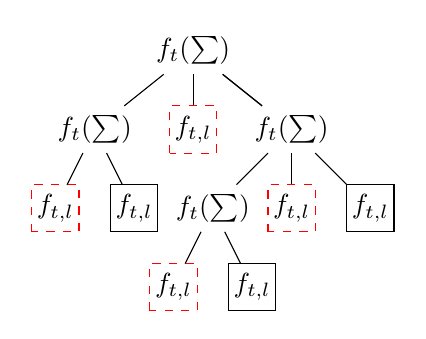
\begin{tikzpicture}
\node (a) at (-.25,0) {$f_{t}(\sum)$};
\node (labela) at (-.25,-1) {$f_{t,l}$};
\node (b) at (-1.5,-1) {$f_{t}(\sum)$};
\node (labelb) at (-2,-2) {$f_{t,l}$};
\node (c) at (-1,-2) {$f_{t,l}$};
\node (d) at (1,-1) {$f_{t}(\sum)$};
\node (labeld) at (1,-2) {$f_{t,l}$};
\node (e) at (0,-2) {$f_{t}(\sum)$};
\node (labele) at (-.5,-3) {$f_{t,l}$};
\node (f) at (2,-2) {$f_{t,l}$};
\node (g) at (.5,-3) {$f_{t,l}$};

\draw (a) -- (labela);
\draw (a) -- (b) -- (c);
\draw (b) -- (labelb);
\draw (d) -- (labeld);
\draw (e) -- (labele);
\draw (a) -- (d) -- (e) -- (g);
\draw (a) -- (d) -- (f);

\draw [red, dashed] (-2.3,-2.3) rectangle (-1.7,-1.7);
\draw (-1.3,-2.3) rectangle (-.7,-1.7);
\draw [red, dashed] (-.55,-1.3) rectangle (.05,-.7);
\draw [red, dashed] (.7,-2.3) rectangle (1.3,-1.7);
\draw (1.7,-2.3) rectangle (2.3,-1.7);
\draw [red, dashed] (-.8,-3.3) rectangle (-.2,-2.7);
\draw (.2,-3.3) rectangle (.8,-2.7);
\end{tikzpicture}
  		\caption{Normalized term frequency computation in the MF ranking for the entity.}
  		\label{fig:mf-ranking}
  	\end{subfigure}
	\caption{Abstract models for ranking a tree.}
	\label{fig:tree}
\end{figure}

\subsection{Eliteness}

In \cite{harter:1974:thesis}, Harter introduced the notion of \emph{eliteness} in order to model content-bearing terms: a document is said to be \emph{elite} in term $t$ if it is somehow ``about'' the topic associated with $t$. In \cite{robertson:1981:PMI}, Robertson et al. introduce the relationship between the eliteness of a term in a document and its frequency: an elite term is most likely to be reused in the document, hence the term frequency is used as evidence of the term eliteness in the document. In \cite{zaragoza:2004:microsoft}, Zaragoza et al. extend the notion of eliteness to documents with multiple fields. In \cite{robertson:2004:cikm}, the authors argue that the normalized frequencies of a term in each field should be combined before applying the term weighting model. Similarly in our MF model, the term eliteness in an entity is shared between its attributes. The values related to a same attribute are associated to a same topic, described by the attribute label. Therefore, a term eliteness in an attribute is shared between its values.

Although values are related to a same attribute, the relevancy of each value with regard to the query is different. We can assume that, given a same attribute, an entity where two terms occur in a single value is more relevant than another entity where each term occurs in two values. This can be seen as a way to integrate some kind of term proximity measure in the retrieval model, i.e., two words are considered close to each other when they occur in the same value. Reflecting this difference into the importance of a term using an appropriate value-specific weight can improve the ranking efficiency.

\section{MF Ranking Functions}
\label{sec:mf-function}

In this section, we describe \emph{BM25MF} and \emph{PL2MF}, the MF extensions of BM25F~\cite{zaragoza:2004:microsoft} and PL2F~\cite{macdonald:2005:clef}, respectively.
We present first the features needed for the MF ranking model and then define both extensions.

\paragraph{Ranking features.}

The MF ranking model requires the following features:
\begin{labeling}{\textbf{average attribute cardinality:}}
  \item[\textbf{leaf length:}] refers to the number of terms in the label of a leaf;
  \item[\textbf{average leaf length:}] is the mean of the siblings \emph{leaf length};
  \item[\textbf{attribute cardinality:}] is equal to the number of values an attribute possesses;
  \item[\textbf{average attribute cardinality;}] is equal to the mean of the \emph{attribute cardinality} across the entities where that attribute appears.
\end{labeling}

\subsection{BM25MF}

BM25F is extended by adapting the Equation (\ref{eq:bm25f_1}). The resulting normalised term frequency is then passed to the term frequency normalisation function in the Equation (\ref{eq:bm25f_2}).
The computation of the entity score with BM25MF consists of applying two functions, $f_{t,l}$ and $f_t$, applied on a leaf and on an internal node, respectively. After applying $f_{t,l}$ on the leaves, the results are summed up on the parent node. Then, this parent node applies the function $f_t$ on the result of the sum. This process is repeated until the root of the tree is reached.
\begin{align}
\label{bm25mf_v}
f_{t,l} & = & \frac{\alpha_v\times f_{t,e,v}}{1+b_v\times\left(\frac{l_{e,v}}{l_a}-1\right)}\\
\label{bm25mf_a}
f_{t} & = & \frac{\alpha_a\times f_{t,c}}{1+b_a\times\left(\frac{\left|{a}\right|_e}{\left|{a}\right|}-1\right)}
\end{align}
in which the following notations are used:
\begin{itemize}
\item $f_{t,e,v}$ is the frequency of the term $t$ within the value $v$ in the entity $e$;
\item $l_{e,v}$ is the \emph{value length} of the value $v$ in the entity $e$;
\item $\left|{a}\right|_e$ is the \emph{attribute cardinality} of the attribute $a$ in the entity $e$;
\item $\left|{a}\right|$ is the \emph{average attribute cardinality} of the attribute $a$;
\item $\alpha_v$ and $\alpha_a$ are respectively value and attribute specific weights; and
\item $b_a$ and $b_v$ are parameters of the term frequency's normalization, where $b_v$ is value-specific and $b_a$ attribute-specific with $(b_a,b_v)\in\left[0,1\right]^2$.
\end{itemize}

\subsection{PL2MF}

PL2F is extended by adapting the Equation (\ref{eq:pl2f}). The resulting normalised term frequency is then passed to the term frequency normalization function (\ref{eq:dfr-prisk}).
The computation of the entity score with PL2MF consists of applying two functions, $f_{t,l}$ and $f_t$, applied on a leaf and on an internal node, respectively. After applying $f_{t,l}$ on the leaves, the results are summed up on the parent node. Then, this parent node applies the function $f_t$ on the result of the sum. This process is repeated until the root of the tree is reached.
\begin{eqnarray}
  \label{eq:pl2mf_v}
  tfn_a & = & \sum_{v\in a}{\alpha_v\times f_{t,e,v} \times log_2\left(1+c_v\times\frac{l_a}{l_{e,v}}\right)}\\
  \label{eq:pl2mf_a}
  tfn & = & \sum_{a\in e}{\alpha_a\times tfn_a \times log_2\left(1+c_a\times\frac{\left|{a}\right|}{\left|{a}\right|_e}\right)}
\end{eqnarray}
where $c_a$ and $c_v$ are hyperparameters, with $c_a$ specific to the attribute $a$ and $c_v$ to the value $v$, with $(c_a,c_v) \in\; ]0,+\infty[^2$.

\minisec{Generalisation}

In Equations (\ref{bm25mf_v}) and (\ref{eq:pl2mf_v}), we normalize the term frequency based on the \emph{average attribute length} $l_a$. In Equations (\ref{bm25mf_a}) and (\ref{eq:pl2mf_a}), we further normalize the term frequency based on the \emph{average attribute cardinality} $\left|{a}\right|$.
In addition to attribute-specific weights $\alpha_a$, the MF ranking model allows value-specific weights in its implementations with the parameter $\alpha_v$. We will present value and attribute specific weights in the next section.

If we assume a single value per attribute to match field-based ranking models, then the Equations (\ref{bm25mf_v}) and (\ref{bm25mf_a}) are transformed into the Equation (\ref{eq:bm25f_2}), with $\alpha_a\times\alpha_v$ as the BM25F's attribute weight, and $b_v$ as the attribute normalization parameter. BM25MF is under this condition equivalent to BM25F. Under the same assumption, the Equations (\ref{eq:pl2mf_v}) and (\ref{eq:pl2mf_a}) are transformed into the Equation (\ref{eq:pl2f}), with $\alpha_a\times\alpha_v\times log_2(1+c_a)$ as the PL2F's attribute weight. PL2MF is under this condition equivalent to PL2F. Therefore, the MF model is a generalisation of field-based models for semi-structured data with multi-valued attributes.
